%----------------------------------------------------------------------------
\chapter{\ManagementExperience}
%----------------------------------------------------------------------------
\section{Rövid szakmai önéletrajz}
%----------------------------------------------------------------------------

A szakmai pályám 2017-ben indult, amikor hangtechnikusként kezdtem dolgozni rendezvényeken, 
elsősorban kisebb koncerteken és kulturális eseményeken. Az évek során egyre több felelősséget vállaltam 
a technikai előkészületek, a helyszíni lebonyolítás és a csapatmunka terén. 2019-ben kaptam lehetőséget arra, 
hogy vezető beosztásban folytassam a munkát hangmérnökként és projektmenedzserként a TéDé Rendezvények csapatában.

Ebben a szerepben fő feladataim közé tartozik a rendezvények technikai tervezése és koordinálása, 
a stáb munkájának irányítása, valamint az ügyfelekkel való folyamatos kommunikáció. 
Egy-egy projekt során 5-15 fős technikai csapatot vezetek, és rendszeresen több párhuzamos esemény 
előkészítéséért és lebonyolításáért felelek. A munkám során gyakran kell gyors döntéseket hozni, 
váratlan helyzeteket kezelni, és közben biztosítani, hogy a technikai minőség és a csapatmorál is 
egyaránt magas szinten maradjon.

%----------------------------------------------------------------------------
\begin{figure}[H]
	\centering
	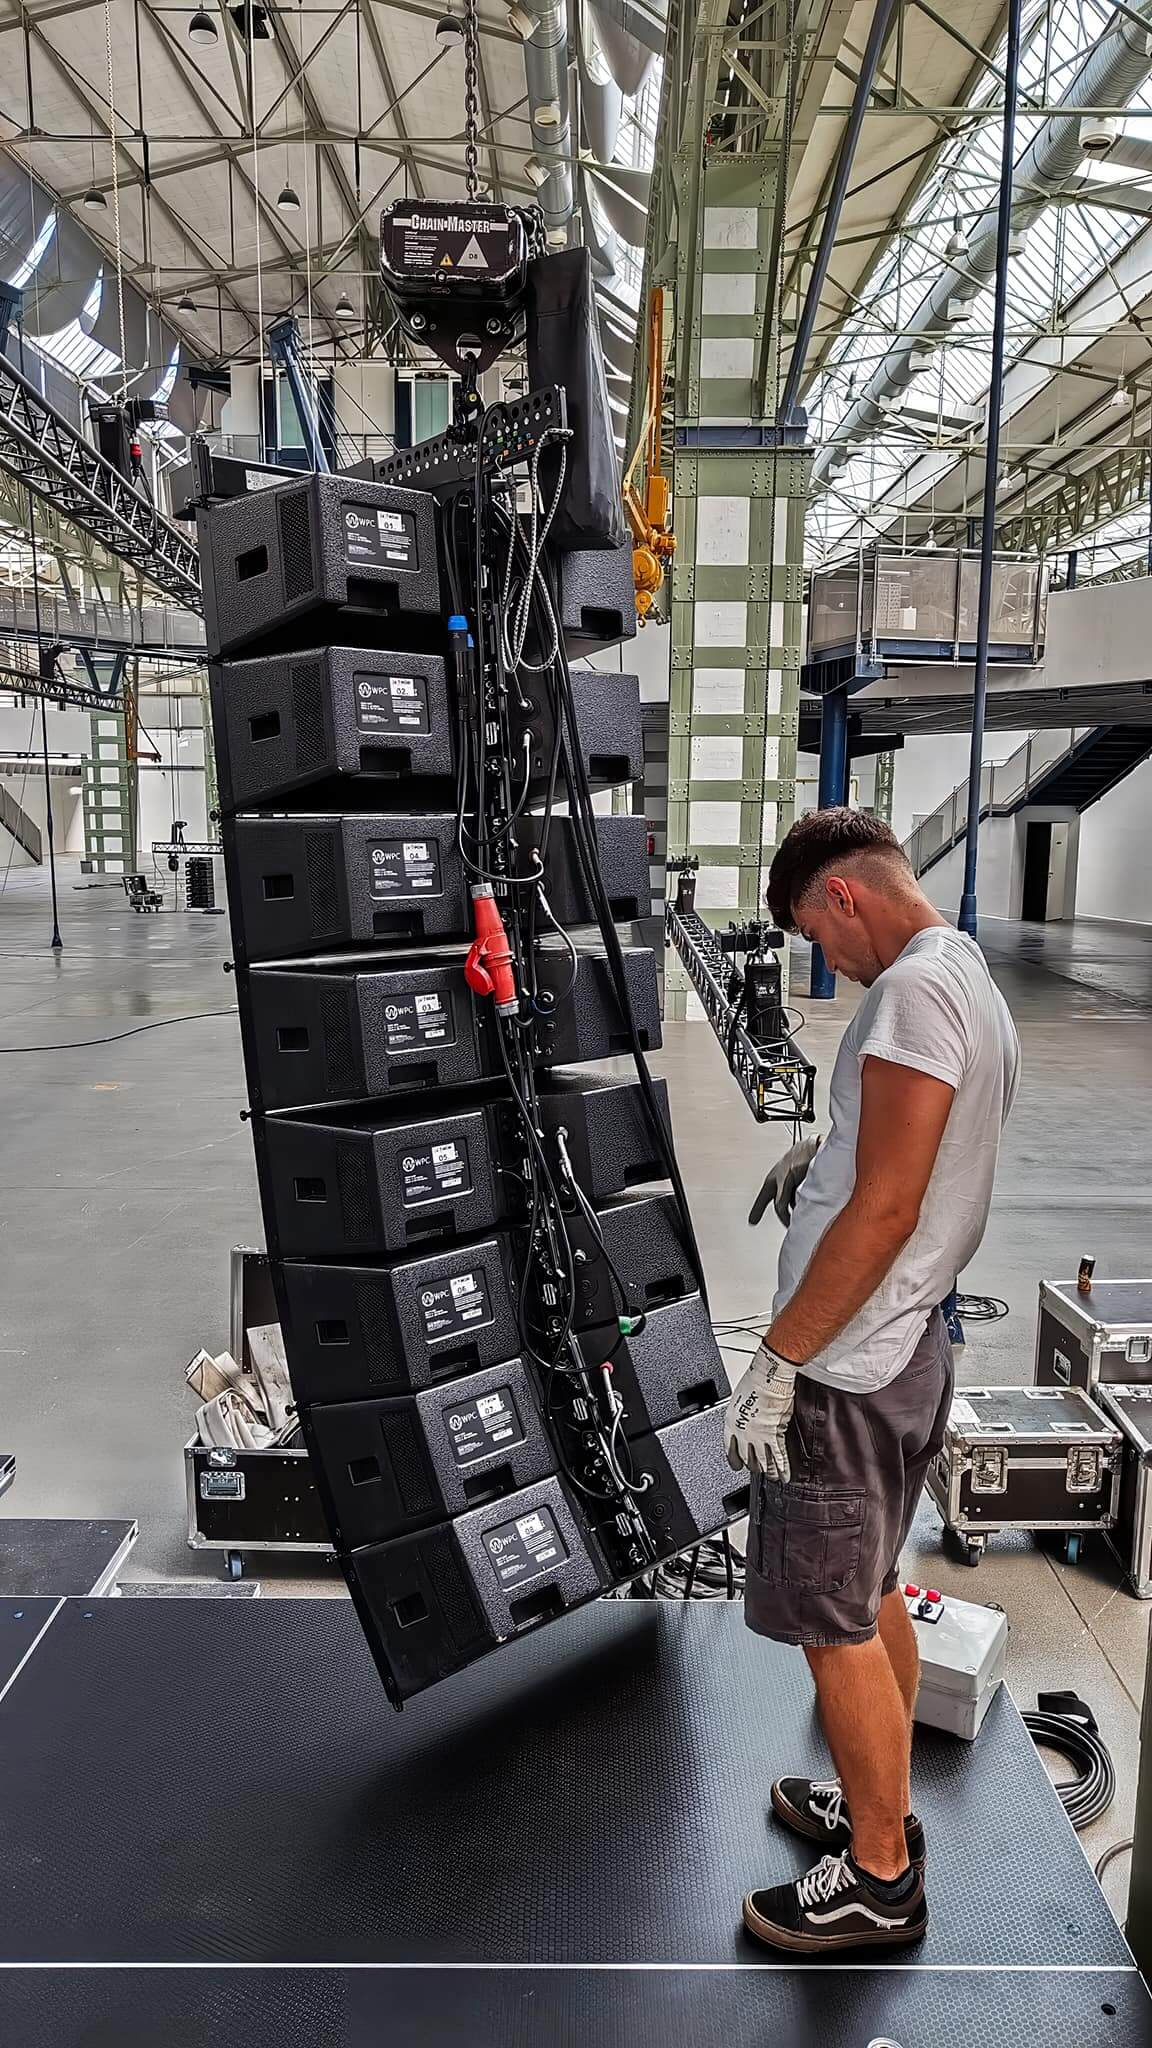
\includegraphics[width=60mm, keepaspectratio]{figures/danci_wpc.jpg}
	\caption{A dolgozat szerzője munka közben}
	\label {fig:danci_wpc}
\end{figure}
%----------------------------------------------------------------------------

%----------------------------------------------------------------------------
\section{A vezetői szerep kialakulása a szakmai fejlődésben}
%----------------------------------------------------------------------------

Vezetővé válásom nem egyik napról a másikra történt. Az első időszakban leginkább a szakmai tudásomra 
támaszkodtam: hangmérnökként pontosan tudtam, mit és hogyan kell megoldani technikailag, 
de a csapat irányítása eleinte sok kihívást tartogatott. Idővel rájöttem, hogy a jó vezetés nem a hibátlan 
szakmai teljesítményről, hanem az emberek megértéséről, motiválásáról és támogatásáról szól.

Meg kellett tanulnom feladatokat delegálni, és bízni abban, hogy a csapatom tagjai felelősen és kreatívan dolgoznak. 
Ezzel párhuzamosan fejlődött a kommunikációs és problémamegoldó képességem, hiszen a rendezvények világa gyakran 
kiszámíthatatlan: váratlan technikai hibák, időnyomás, vagy akár ügyféloldali változtatások is előfordulhatnak. 
Ilyen helyzetekben megtanultam nyugodtnak maradni, priorizálni és gyorsan dönteni - ami mára az egyik legerősebb 
vezetői kompetenciámmá vált.

Ugyanakkor azt is felismertem, hogy vannak olyan területek, ahol folyamatosan fejlődnöm kell. 
Ilyen például a stratégiai gondolkodás és a hosszú távú tervezés, mivel a rendezvényiparban gyakran a napi operatív 
feladatok viszik el az energiát. A dolgozatban bemutatott önértékelő teszt és a hozzá kapcsolódó elemzések 
segítenek abban, hogy ezeket a fejlesztendő kompetenciákat tudatosabban lássam és célzottan dolgozzak rajtuk.
